%%%%%%%%%%%%%%%%%%%%%%%%%%%%%%%%%%%%%%%%%%%%%%%%%%%%%%%%%%%%%%%%%%%%%%%%%%%%%%%
%     STYLE POUR LES EXPOSÉS TECHNIQUES 
%         3e année INSA de Rennes
%
%             NE PAS MODIFIER
%%%%%%%%%%%%%%%%%%%%%%%%%%%%%%%%%%%%%%%%%%%%%%%%%%%%%%%%%%%%%%%%%%%%%%%%%%%%%%%

\documentclass[a4paper,11pt]{article}

%\usepackage{biblatex}
\usepackage{lipsum}
\usepackage{titling}
\usepackage{exptech}       % Fichier (./exptech.sty) contenant les styles pour 
                           % l'expose technique (ne pas le modifier)

\usepackage{pgfplots}
\pgfplotsset{compat=1.13}

%\linespread{1,6}          % Pour une version destinée à un relecteur,
                           % décommenter cette commande (double interligne) 
                           
% UTILISEZ SPELL (correcteur orthographique) à accès simplifié depuis XEmacs

%%%%%%%%%%%%%%%%%%%%%%%%%%%%%%%%%%%%%%%%%%%%%%%%%%%%%%%%%%%%%%%%%%%%%%%%%%%%%%%

\title{ \textbf{Apprentissage incrémental de règles de décision} }
\markright{\thetitle} 
                           % Pour avoir le titre de l'expose sur chaque page

\author{Bassirou \textsc{Seye}, Clément \textsc{Fournier}, \\
        Léandre \textsc{Le Polles -{}- Potin}, Pierre \textsc{Testart} \\
        \\
        Encadreur : Laurence \textsc{Rozé}}

\date{}                    % Ne pas modifier
 
%%%%%%%%%%%%%%%%%%%%%%%%%%%%%%%%%%%%%%%%%%%%%%%%%%%%%%%%%%%%%%%%%%%%%%%%%%%%%%%

\def\antd#1{\texttt{#1}}


\begin{document}          

    \maketitle                 % Génère le titre
    \thispagestyle{empty}      % Supprime le numéro de page sur la 1re page

    \begin{abstract}
        Notre projet a eu pour but de nous faire implémenter l’algorithme VFDR, en nous servant de l’API de Weka. Cet algorithme est décrit dans le document de recherche intitulé “Learning decision Rules from Data Streams” de João Gama et Petr Kosina.

    \end{abstract} 

    \section{Introduction}

    \subsection{Notions d'apprentissage artificiel}

        Pour introduire les notions principales nécessaires à la compréhension du travail accompli, nous allons prendre un exemple qui nous servira de fil directeur : l’exemple classique de la différentiation entre les oies et les cygnes. La question posée est la suivante : “Comment un programme peut-il différencier ces deux oiseaux ?”.

        \subsubsection{Règles de décisions}

            La classification est une tâche qui consiste à attribuer une étiquette à un individu donné en entrée. Notre exemple des oiseaux est un exemple de classification: à partir de données sur un oiseau, on doit déterminer si c'est une oie ou un cygne. Dans les algorithmes qui apprennent des règles, on base la décision d'attribuer une étiquette particulière à l'individu sur la validation de certaines "règles," c'est à dire la réalisation simultanée d'une ou plusieurs conditions sur les données qui décrivent l'individu à classifier.

            Les données qui décrivent chaque individu sont les valeurs associées à des caractéristiques mesurables de l'individu, qu'on appelle des \emph{attributs}. Par exemple, pour nos oiseaux, la taille en centimètre est un attribut numérique (sa valeur est un nombre) et la couleur du plumage est un attribut nominal (il prend ses valeurs dans un ensemble fini, par exemple "clair", "moyen" ou "sombre"). Les attributs nominaux et numériques sont les deux types de données que notre algorithme supporte.

            Les règles qui nous permettent de prendre une décision de classification se présentent sous la forme de conjonctions de conditions sur les attributs de l'individu à classifier. On appelle ces conditions des \emph{littéraux} (ou \emph{antécédents}). Sur des attributs numériques, on compare la valeur avec des valeurs seuils, ainsi un antécédent numérique pourrait être \antd{taille > 50cm}. Les valeurs des attributs nominaux ne sont pas ordonnées, les antécédents nominaux sont donc de la forme \antd{plumage = clair}.

            Une règle possible pour classifier les oiseaux est « Si plumage = "clair" et taille > 80, alors classe = "cygne". » On voit donc que si les conditions de la règle sont réunies, on prend une décision de classification. Le but d'un algorithme de classification va être de consituer un ensemble de règles qui décrive au mieux les individus déjà observés pour avoir une estimation de la classe d'un nouvel individu à classifier. C'est le principe simplifié de l'apprentissage de règles.

        \subsubsection{Apprentissage}

            L’apprentissage de règles consiste à laisser l’algorithme définir seul les règles de décisions en lui fournissant un ensemble d’apprentissage, constitué d’individus dont la classe est déjà connue. En fournissant un jeu de données d’individus déjà étiquetés à l’algorithme, celui-ci pourrait par exemple répartir les individus sur un diagramme tel que celui-ci : 

            Et en déduire l’ensemble de règles suivant : 
            « Si plumage = "clair" et taille > 80, alors classe = "cygne"
            Si plumage = "foncé" et taille > 97, alors classe = "cygne"
            Si plumage = "noir", alors classe = "oie"
            Sinon classe = "oie" »


        \subsubsection{Incrémentalité}

            Les algorithmes d’apprentissage incrémentaux sont capables de mettre à jour les règles de décisions à chaque individu catégorisé qu’on lui fournit, tout en laissant la possibilité à tout moment d’utiliser lesdites règles de décisions pour classifier un individu dont on ne connaît pas encore la classe.

            Ces algorithmes sont conçus pour optimiser leur utilisation d'espace mémoire et le temps qu'ils mettent à classifier une instance, et sont donc adaptés à l'apprentissage sur des flux de données importants et continus.

    \subsection{Weka}

        Weka (Waikato Environment for Knowledge Analysis) est une plate-forme d'apprentissage artificiel, programmée en Java, permettant de réaliser de nombreuses tâches d’apprentissage et de classification. Elle rend accessible les différentes techniques de Data Mining et de Machine Learning et  permet d’appliquer rapidement ces techniques sur des problèmes concrets.

    \subsection{Présentation de VFDR}

        L’algorithme VFDR, sigle de "Very Fast Decision Rules," est l’algorithme d’apprentissage incrémental de règles qui nous intéressera ici. Nous allons dans ce chapitre décrire le fonctionnement de cet algorithme.

        \subsubsection{Principe}

            L’algorithme commence avec un ensemble vide de règles et une règle par défaut. Cette règle, ne comprenant aucun littéral, pourrait être exprimé par “Sinon …” comme dans l’exemple d’ensemble de règle ci-dessus. A chaque règle est associée une structure de donnée permettant de calculer les statistiques nécessaire pour le traitement de ladite règle.

            Si tous les littéraux d’une règle sont vrai pour un individu donné, on dit qu’il est \emph{couvert} par cette règle. Lorsque l’algorithme reçoit un individu étiqueté, il tente de le faire correspondre à chaque règle de l’ensemble de règles créés ou à la règle par défaut. Si la règle qui le couvre contient suffisamment d’individus, elle est étendue pour améliorer sa précision. L’extension d’une règle consiste à lui rajouter un littéral. Lorsque c’est la règle vide qui devrait être étendue, une nouvelle règle est créée à la place. Ainsi, l’algorithme crée l’ensemble de règle qui servira à classifier les individus non étiquetés.

        \subsubsection{Description des statistiques}

            Pour ne pas saturer la mémoire, l’algorithme n’enregistre pas l’ensemble des individus traités, mais utilise une structure de donnée permettant de calculer les statistiques pertinentes liée à chaque règle. Cette structure de données est composée de : 
            \begin{itemize}
                \item Un entier, correspondant au nombre d’individus couverts par la règle.
                \item Un vecteur d’entier, comprenant le nombre d’occurence de chaque classe parmis les individus couverts.
                \item Une matrice, représentant le nombre d'occurrence de chaque valeur des attributs nominaux pour chaque classe.
                \item Un estimateur gaussien, permettant de calculer pour chaque attribut numérique la probabilité de rencontrer une valeur supérieur à telle ou telle valeur déjà rencontrée, par classe.
            \end{itemize}

        \subsubsection{Expansion d'une règle}
        \subsubsection{Concept de règle non-décisionnelle}





    \section{Travail réalisé}

    \subsection{Organisation} 

        Notre objectif pour ce second semestre d’étude pratique était d’implémenter l’algorithme. Nous avons décidé de travailler chacun de notre côté dans un premier temps, car nous ne connaissions pas suffisamment le fonctionnement de Weka, et le travail semblait difficilement sécable. Cette approche nous a effectivement permis de nous familiariser individuellement avec la bibliothèque Weka, et nous avons chacun travaillé sur un début d’implémentation de VFDR.

        Nous nous sommes ensuite réunis pour comparer nos avancées respectives, et nos choix d’implémentation. Nous avons décidé de conserver les choix faits par Clément, qui avait déjà bien avancé dans l’implémentation de l’algorithme. C’est donc la base que nous avons choisie pour terminer le travail du semestre.

    \begin{figure}

        \includegraphics[width=\textwidth]{SOURCES/image2}
        \caption{Diagramme de classes de notre implémentation}
        \label{fig:dclass}
    \end{figure}


    \subsection{Description de l'implémentation}

        Le diagramme de classes en figure \ref{fig:dclass} présente l'architecture de notre implémentation.

        \paragraph{Paramétrage} La classe principale de notre programme, nommée \texttt{Vfdr}, implémente plusieurs interfaces de Weka, notamment UpdateableClassifier, qui permet de mettre en avant l’aspect incrémental de l’algorithme. Ces interfaces permettent d'intégrer le programme au GUI de Weka. \texttt{Vfdr} possède des attributs servant d’options de configuration, ainsi qu’une liste de \texttt{VfdrRule}, représentant l’ensemble des règles, et une \texttt{VfdrRule} à part, qui est la règle par défaut.

        \paragraph{Règles}Chaque objet \texttt{VfdrRule} possède lui-même une liste d’\texttt{Antd}, une classe abstraite servant à représenter les antécédents possibles pour les règles (spécialisée en \texttt{NumericAntd} pour les conditions sur les attributs numériques, et \texttt{NominalAntd} pour les conditions sur les attributs nominaux). \texttt{VfdrRule} possède aussi une référence vers un objet \texttt{SufficientStats}, qui stocke les statistiques associées à la règle. 


        \paragraph{Statistiques suffisantes} 
            Dans l’implémentation, nous avons choisi d’identifier les classes des exemples par des Strings (le nom de la classe). Par conséquent, dans \texttt{SufficientStats}, le nombre d’exemples couverts par classe est stocké dans une \texttt{Map<String, Integer>}. Pour ce qui est des attributs, ils peuvent être représentés par des entiers (leur indice). On utilise par exemple une \texttt{List<Integer>} pour stocker les attributs déjà utilisés dans \texttt{SufficientStats}. Cependant, les attributs sont parfois identifiés par leur nom, comme les classes : les statistiques par attributs sont stockés dans une \texttt{Map<String, \texttt{AttributeStats}>}, où \texttt{AttributeStats} est une classe abstraite qui a des spécialisations différentes selon le type d’attribut.
            
            Pour gérer les statistiques des attributs numériques, certaines descriptions de \texttt{VFDR} indiquent d’utiliser un arbre binaire qui stocke pour chaque attribut la chance de rencontrer une valeur supérieure à chaque valeur déjà rencontrée. Pour simplifier l’implémentation, nous avons plutôt utilisé une densité de probabilité pour représenter les valeurs rencontrées : c’est la classe \texttt{GaussianAttributeStats}, qui hérite de \texttt{AttributeStats}. Les calculs sont faits dans la classe interne \texttt{GaussianEstimator}, qui hérite de la classe Weka \texttt{UnivariateNormalEstimator}. Ce choix a aussi l’avantage de limiter la complexité en temps et en espace.
        
        \paragraph{Expansion d'une règle} Pour l’expansion d’une règle, une liste de \texttt{CandidateAntd} (antécédents candidats) est créée. Le score de chaque candidat est évalué à l’aide d’un objet \texttt{ExpansionMetric}. Notons qu’\texttt{ExpansionMetric} est une classe abstraite, mais qu’elle n’a qu’une seule spécialisation possible : \texttt{Entropy}, qui utilise des calculs d’entropie pour évaluer la qualité d’une séparation. La mise en place d’une classe abstraite permet de laisser la possibilité d’améliorer l’implémentation, en ajoutant des méthodes d’évaluation de séparation, en limitant les modifications à apporter au code existant.
        
        \paragraph{Prédiction} Lorsque l’on demande au \texttt{Vfdr} de classifier un exemple via la méthode \texttt{distributionForInstance}, sa stratégie de classification (représentée par la classe abstraite ClassificationStrategy) entre en jeu. Pour les ensembles ordonnés de règles, la stratégie est de type FirstHit, on renvoie la classe donnée par la première règle qui couvre l’exemple. Pour les ensembles non ordonnés, la stratégie est de type WeightedMax, on choisit alors la classe à partir de la règle qui couvre l’exemple et a le poids le plus élevé (le plus grand nombre total d’exemples couverts).

    \subsection{Limites de cette implémentation}

        Pas trop de problèmes avec la mémoire, car tous les exemples ne sont pas mémorisés, on conserve des statistiques suffisantes. Il y a seulement une augmentation possible du nombre de règles, qui prendraient plus de place mémoire.

        Au niveau de la complexité en temps : le plus problématique est la détermination d’antécédent pour étendre une règle. Il faudrait regarder la complexité exacte des opérations. Faire remarquer qu’on met en place un seuil minimal avant d’étendre la règle, justement à cause du temps de calcul élevé.
        
        Autres limites de l’algo : les types de données gérés. La classe est forcément un attribut nominal.
        
        L’algorithme ne gère pas le concept drift (une variante de l’algorithme qui le gère existe, mais nous ne l’avons pas implémentée dans ce projet).

    \subsection{Comparaison avec un autre algorithme: VFDT}

        Dans le domaine du machine learning, surtout dans les tâches de classification les arbres de décisions (tels que VFDT) sont très largement utilisés. Ils ont l’avantage d’être lisibles avec une structure hiérarchique où les  feuilles de l’arbre représentent les différentes décisions possibles et sont atteints en fonction des décisions prises à chaque étape. Ils ont également de bonnes capacités prédictives. Par ailleurs, tout arbre de décision peut être facilement transformé en une collection de règles. Chaque règle correspond au chemin de la racine à une feuille, et il y a autant de règles que de feuilles. Ce processus génère un ensemble  de règles avec la même complexité qu’un arbre de décision. 

        Le VFDT (Very Fast Decision Tree) est l’un des algorithmes de classification incrémentale les plus connus. Cet algorithme peut automatiquement s’adapter à l’évolution des données au cours du temps. Par ailleurs lorsque les données changent au cours du temps, cette adaptation devient de plus en plus lente et pénible pour un arbre de décision dans la mesure où dans certains cas il faudrait reconstruire le classifieur à partir de zéro ou exécuter un changement complexe dans la structure de l’arbre. Par contre, un algorithme comme VFDR a une capacité à s’adapter beaucoup plus facilement avec les changements que peuvent subir les données. Ils ont l’avantage d’avoir des règles individuelles qui peuvent être gérées de manière indépendante. L’ensemble de règles peut être donc plus facilement modifié : les règles obsolètes peuvent être tout simplement supprimées. 
    \section{Travail réalisé}

    \subsection{Organisation} 

        Notre objectif pour ce second semestre d’étude pratique était d’implémenter l’algorithme. Nous avons décidé de travailler chacun de notre côté dans un premier temps, car nous ne connaissions pas suffisamment le fonctionnement de Weka et le travail semblait difficilement sécable. Cette approche nous a effectivement permis de nous familiariser individuellement avec la bibliothèque Weka et nous avons chacun travaillé sur un début d’implémentation de VFDR.

        Nous nous sommes ensuite réunis pour comparer nos avancées respectives et nos choix d’implémentation. Nous avons décidé de conserver les choix faits par Clément, pour des raisons de conception. C’est donc la base que nous avons utilisée pour terminer le travail du semestre.

    \begin{figure}
        \includegraphics[width=\textwidth]{src/image2}
        \caption{Diagramme de classes de notre implémentation}
        \label{fig:dclass}
    \end{figure}


    \subsection{Description de l'implémentation}

        Le diagramme de classes en figure \ref{fig:dclass} présente l'architecture de notre implémentation.

        \paragraph{Paramétrage} La classe principale de notre programme, nommée \texttt{Vfdr}, implémente plusieurs interfaces de Weka, notamment \texttt{UpdateableClassifier}, qui permet de mettre en avant l’aspect incrémental de l’algorithme. Ces interfaces permettent d'intégrer le programme au GUI de Weka. \texttt{Vfdr} possède des attributs servant d’options de configuration, ainsi qu’une liste de \texttt{VfdrRule}, représentant l’ensemble des règles et une \texttt{VfdrRule} à part qui est la règle par défaut.

        \paragraph{Règles}Chaque objet \texttt{VfdrRule} possède lui-même une liste d’\texttt{Antd}, une classe abstraite servant à représenter les antécédents possibles pour les règles (spécialisée en \texttt{NumericAntd} pour les conditions sur les attributs numériques et \texttt{NominalAntd} pour les conditions sur les attributs nominaux). \texttt{VfdrRule} possède aussi une référence vers un objet \texttt{SufficientStats}, qui stocke les statistiques associées à la règle. 


        \paragraph{Statistiques suffisantes} 
            Dans l’implémentation, nous avons choisi d’identifier les classes des exemples par des Strings (le nom de la classe). Par conséquent, dans \texttt{SufficientStats}, le nombre d’exemples couverts par classe est stocké dans une \texttt{Map<String, Integer>}. Pour ce qui est des attributs, ils peuvent être représentés par des entiers (leur indice). On utilise par exemple une \texttt{List<Integer>} pour stocker les attributs déjà utilisés dans \texttt{SufficientStats}. Cependant, les attributs sont parfois identifiés par leur nom, comme les classes : les statistiques par attributs sont stockés dans une \texttt{Map<String, \texttt{AttributeStats}>}, où \texttt{AttributeStats} est une classe abstraite qui a des spécialisations différentes selon le type d’attribut.
            
            Pour gérer les statistiques des attributs numériques, certaines descriptions de l'algorithme VFDR indiquent d’utiliser un arbre binaire qui stocke pour chaque attribut la chance de rencontrer une valeur supérieure à chaque valeur déjà rencontrée. Pour simplifier l’implémentation, nous avons plutôt utilisé une densité de probabilité pour représenter les valeurs rencontrées : c’est la classe \texttt{GaussianAttributeStats}, qui hérite de \texttt{AttributeStats}. Les calculs sont faits dans la classe interne \texttt{GaussianEstimator}, qui hérite de la classe Weka \texttt{UnivariateNormalEstimator}. Ce choix a aussi l’avantage de limiter la complexité en temps et en espace.
        
        \paragraph{Expansion d'une règle} Pour l’expansion d’une règle, une liste de \texttt{CandidateAntd} (antécédents candidats) est créée. Le score de chaque candidat est évalué à l’aide d’un objet \texttt{ExpansionMetric}. Notons qu’\texttt{ExpansionMetric} est une classe abstraite, mais qu’elle n’a qu’une seule spécialisation possible : \texttt{Entropy}, qui utilise des calculs d’entropie pour évaluer la qualité d’une séparation. La mise en place d’une classe abstraite permet de laisser la possibilité d’améliorer l’implémentation, en ajoutant d'autres méthodes d’évaluation de séparation, tout en limitant les modifications à apporter au code existant.
        
        \paragraph{Prédiction} Lorsque l’on demande au \texttt{Vfdr} de classifier un exemple via la méthode \texttt{distributionForInstance}, sa stratégie de classification (représentée par la classe abstraite \texttt{ClassificationStrategy}) entre en jeu. Pour les ensembles ordonnés de règles, la stratégie est de type \texttt{FirstHit}, on renvoie la classe donnée par la première règle qui couvre l’exemple. Pour les ensembles non ordonnés, la stratégie est de type \texttt{WeightedMax}, on choisit alors la classe à partir de la règle qui couvre l’exemple et a le poids le plus élevé (le plus grand nombre total d’exemples couverts).

    \subsection{Limites de cette implémentation}

        Le temps de traitement d'un individu est suffisamment bas pour qu'il ne constitue pas un problème. Cependant la routine d'expansion de règle est très coûteuse et constitue le principal goulot d'étranglement pour le temps d'exécution du programme. Pour cette raison, nous avons défini une borne inférieure au nombre d'exemples que l'algorithme doit voir passer avant de tenter l'expansion. Cette limite est configurable et doit être adaptée au nombre d'exemples de l'échantillon d'apprentissage.

        L’algorithme ne peut pas gérer de changement de la fonction cible (ce que l'on appelle la \emph{dérive de concept}). Il existe une variante de l'algorithme qui peut s'y adapter, mais son implémentation était hors du champ de cette étude pratique.

        

    \section{Conclusion} 
%        \lipsum[2]

    \nocite{*}
    \bibliography{biblio}


\end{document}
